\documentclass[UKenglish]{scrreprt}

\RequirePackage[numbers, round]{natbib}
\RequirePackage[utf8]{inputenc}              % Direkte Eingabe von ä usw.
\RequirePackage[T1]{fontenc}                 % Font Kodierung für die Ausgabe        
\RequirePackage{babel}                       % Verschiedenste sprach-spezifische Extras
\RequirePackage[autostyle=true]{csquotes}    % Intelligente Anführungszeichen
\RequirePackage{graphicx}                    % zum Bilder einbinden
\RequirePackage[]{amssymb}                   %
\RequirePackage{amsmath}                     %Mathekram
\RequirePackage{physics}                     %Für Einheiten und so
\RequirePackage{hyperref}                    %
\RequirePackage[all]{hypcap}                 %
\usepackage{siunitx}
\RequirePackage{newtxmath}                   % Schönere Schriftart
\RequirePackage{newtxtext}                   % Schönere Schriftart    
\KOMAoptions{fontsize=11pt, paper=a4}        % Schriftgröße und Papierformat setzen
\KOMAoptions{DIV=11}                         % Parameter mit dem man den Seitenrand ändern kann
\KOMAoptions{listof=totoc}                   % Abbildungs- und Tabellenverzeichnis im Inhaltverzeichnis  aufzuführen


\title{Where should I go? Finding the optimal neighborhood in Bonn to move to from Munich}
\subtitle{IBM Applied Data Science Capstone Project}
\author{Laila Linke}
\date{\today}

\begin{document}

\maketitle

%\chapter*{Executive summary}
%
%\paragraph{Key question:}In this report, we answer the following key question: \emph{Which neighborhoods in the German city Bonn are most similar to the cite centre of Munich?} This question is relevant for people, who plan to move from Munich to Bonn and want to choose their new neighborhood to have similar stores, amenities, and restaurants as their current living place. 
%
%\paragraph{Data \& Methodology:}We tackle this question with data on the location and category of venues from Foursquare, as well as publicly available location data from the city council of Bonn. Using this data, we find the most common venue categories for each neighborhood in Bonn and compare these to the most common venues near the University of Munich. We also cluster similar neighborhoods in Bonn using the k-means clustering algorithm and find the neighborhood cluster in Bonn that is closest to Munich. 
%
%\paragraph{Results:}Our results are
%\begin{itemize}
%	\item The neighborhood most similar to the city centre of Munich is \emph{Bonn-Zentrum}.
%	\item The neighborhood cluster most similar to Munich consists of primarily of areas at the river Rhine.
%	\item The neighborhoods \emph{Ückesdorf} and \emph{Küdinghoven} are the most dissimilar to Munich
%\end{itemize}
%
%\paragraph{Recommendations:}Based on these results we recommend a person moving from Munich to Bonn to \emph{move preferably to Bonn-Zentrum} and to \emph{avoid moving to Ückesdorf}.

\chapter{Introduction}
\section{Background}
Bonn and Munich are two German cities, that on the first glance are quite dissimilar. Munich is a big metropolis with \num{1485671} inhabitants\footnote{as of 30th September 2020 }\cite{muenchen}, while Bonn has only \num{329673} \footnote{as of 30th September 2019}
\cite{bonn}. Due to the different population numbers, it is only expected, that different kinds of restaurants, stores, and leisure amenities exist in those two cities. For example, based on the number of inhabitants we would expect the smaller town of Bonn to have less variety in international cuisine. 

However, this is not necessarily the case for all of Bonn. Bonn is divided into 51 different neighborhoods, whose structure and population varies. For example, the area near the Rhine contains international embassies and offices of the United Nations. Therefore, these areas to be more international and have more amenities than the \enquote{average} neighborhood in Bonn.

For a person moving to Bonn, this variety between the neighborhoods poses a problem: Which neighborhood should they choose, so that the restaurants, stores and other venues near them fulfill their expectations? This is exactly the problem we are studying in this report.

\section{Problem}
We are investigating the following problem. A person, currently living in the \emph{Kaulbachstraße} next to the main building of Munich University is planning a move from their current home to Bonn. They enjoy the amenities and variety of venues in their current neighborhood and therefore want to move to a neighborhood with a similar structure. Our goal is to recommend the neighborhoods best suited to this person. 

\section{Proposed methodology}% and structure of this report}

To solve the problem, we study the venues in each of Bonns neighborhood and compare them to venues near the current home in Munich. We find the most common categories of venues per neighborhood and use them to define the similarity between each of Bonn's neighborhoods and Munich. Based on this similarity, we recommend which neighborhood the person from Munich should move to, and which they should avoid.

Our analysis consists of three parts. In the first part we qualitatively explore the data, by finding the most common venue categories per neighborhood. In the second part we quantify the similarity of each neighborhood with the Munich area and find the single most similar neighborhood. In the third part we group alike neighborhoods into clusters and find the cluster of neighborhoods most similar to Munich.
%
%This report is structured as follows: In Section \ref{sec:Data} we introduce the data sets we used.  Section \ref{sec:Analysis} details our analysis of the data. This analysis includes an exploratory assessment of the most common venue categories per neighborhood (Sect. REF), the determination of the similarity of each neighborhood in Bonn to Munich (Sect. REF), and the ranking of neighborhood clusters according to their similarity to Munich (Sect. REF). The results of our analysis are presented in Section REF and discussed in Section REF. We present our final recommendations and directions for future exploration in Section REF.
%
%The full code for our analysis is available as a Jupyter Notebook under ...

\chapter{Data}
\label{sec:Data}

\section{Used Datasets and -sources}
In this analysis, we require data on the positions of Bonn's neighbourhoods, as well as on the location and category of amenities, restaurants, stores, and other facilities in Bonn and near the current home in Munich. We describe our two data sets in the following.

\subsection{Location and centre of Bonn's neighbourhoods}
We use the location and borders of Bonn's neighbourhoods provided by the city administration on their open data platform \footnote{\href{https://opendata.bonn.de/dataset/fl\%C3\%A4chen-der-ortsteile}{https://opendata.bonn.de/dataset/fl\%C3\%A4chen-der-ortsteile}}\cite{Ortsteile}. This data is available as a GeoJSON file and contains the name, ID and polygon shape of each of the 51 neighbourhoods (in German: \enquote{Stadtteile}), as well as their respective city district and district ID.
The data was first published on 11th February 2015 and is updated daily. It is available publicly under a Creative Commons CC Zero License, meaning that 
it is in the Public Domain and can be freely used and shared for any purpose.

We access the data with the python package \verb|geopandas|\footnote{\href{https://geopandas.org/}{https://geopandas.org/}} and read it into a data frame, whose first five rows are shown in Table REF. We can also visualize the location of Bonn's neighbourhoods, using the \verb|folium| package \footnote{\href{https://python-visualization.github.io/folium/}{https://python-visualization.github.io/folium/}}. The resulting map is shown in Fig.~\ref{fig:map neighbourhoods}.

\begin{figure}[htbp]
	\centering
	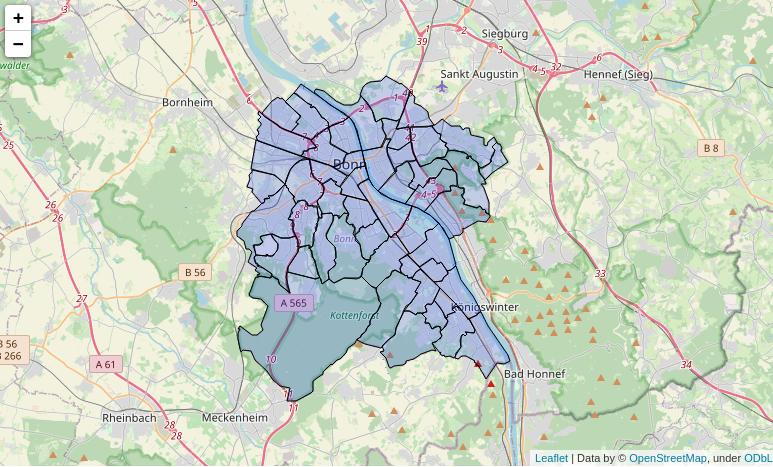
\includegraphics[width=\textwidth]{Figs/Map_Neighborhoods.png}
	\caption{Map of Bonn with neighborhoods overlayed in blue. Location and shape of neighborhoods is from \cite{Ortsteile}, the map of Bonn was created with \texttt{folium}.}
	\label{fig:map neighborhoods}
\end{figure}

To simplify our analysis, we drop the columns describing the neighbourhood ID, the district name, and the district ID from this data frame, as these are not related to our analysis. We also find the centre of each neighbourhood using the \verb|centroid| method of \verb|geopandas| data frames and add the longitude and latitude of the centres to the data frame as new columns.

\subsection{Location and categories of venues}
To obtain the location and categories close to the Munich address and in each neighbourhood in Bonn, we use Foursquare. 
Foursquare is a search and discovery mobile app that provides users with the opportunity to find new venues close to them, recommend and review visited venues and \enquote{check-in} at their favourite places. Due to the app's popularity, Foursquare has obtained a large dataset of the location, category and rating of venues like restaurants, stores, and leisure amenities all over the world. This dataset is accessible via an Application Programm Interface (API), which we are using for our analysis.
Using the Foursquare API and data commercially requires a paid subscription. However, here we are only considering personal use, which is free. 

We use the API to obtain the name, location and category of each venue listed on Foursquare within 500 m of the centre of each of Bonn's neighbourhoods and the Kaulbachstraße in Munich. From the API we obtain 433 venues in Bonn, most of which are supermarkets, and 38 in Munich, most of which are cafés. 

To visually inspect the data, we display the venues along with the neighbourhood centres in Bonn, and the address in Munich in Figs \ref{fig:map venues_bonn} and \ref{fig:map venues_munich}. This inspection shows that there are six neighbourhoods, which do not have any listed venues (Röttgen, Schweinheim, Heiderhof, Geislar, Brüser Berg and Holzlar). Our analysis, therefore, cannot apply to these neighbourhoods.

\begin{figure}[htbp]
	\centering
	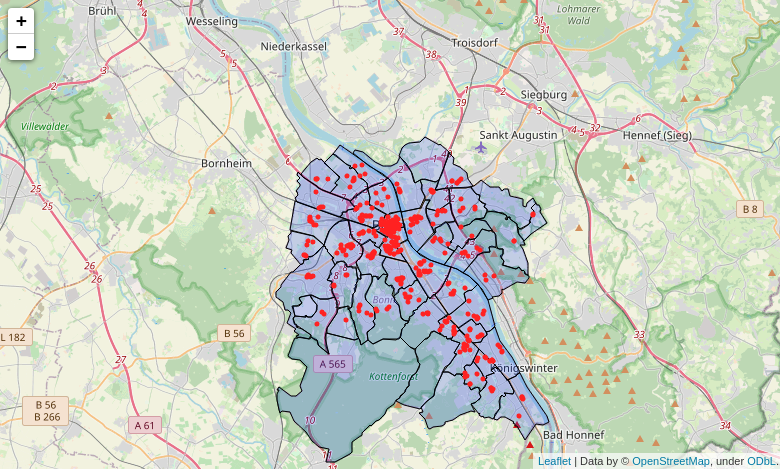
\includegraphics[width=\textwidth]{Figs/Map_Bonn_venues.png}
	\caption{Map of venues in Bonn (red circles) around neighborhoods centers (blue circles).}
	\label{fig:map venues_bonn}
\end{figure}

\begin{figure}[htbp]
	\centering
	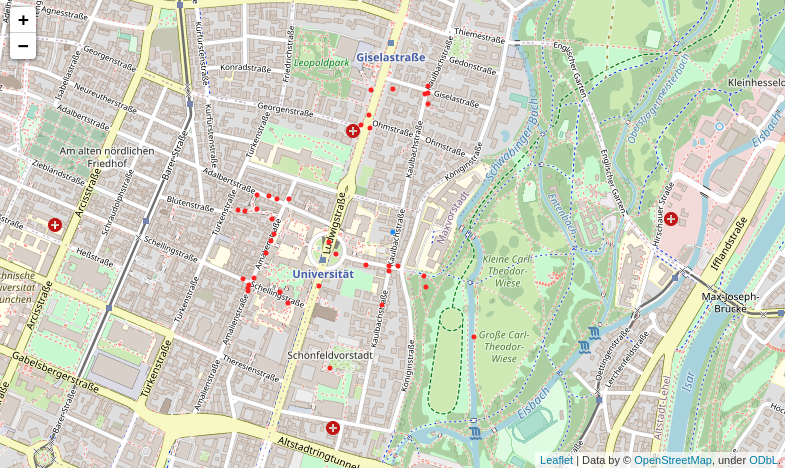
\includegraphics[width=\textwidth]{Figs/Map_Munich_venues.png}
	\caption{Map of venues in Munich (red circles) around current address (blue circle).}
	\label{fig:map venues_munich}
\end{figure}
 
%\chapter{Analysis}
%\label{sec:Analysis}
%Our analysis consists of three parts. In the first part we qualitatively explore the data, by finding the most common venue categories per neighborhood. In the second part we quantify the similarity of each neighborhood with the Munich area and find the single most similar neighborhood. In the third part we group alike neighborhoods into clusters and find the cluster of neighborhoods most similar to Munich.
%\section{Exploratory Data Analysis}
%In our exploratory analysis, we find the most common venue categories per neighborhood. For this, we first calculate the fraction of each venue category per neighborhood. The fraction of the venue category $i$ per neighborhood $j$ is given by
%\begin{equation}
%	f_{ij}=\frac{N_{ij}}{\sum_k N_{kj}}\;,
%\end{equation} 
%where $N_{ij}$ is the number of venues of category $i$ in neighborhood $j$, and the sum goes over all different venue categories. The higher this fraction, the more venues of a specific category are in a neighborhood.
%
%For each neighborhood and the Munich area, we sort the venue categories by their fraction and find the three most common categories.
%
%\section{Determination of most similar neighborhood}
%To determine the most similar neighborhood to Munich, we define the \emph{dissimilarity} $d_{ij}$ of two areas $i$ and $j$ as
%\begin{equation}
%	d_{ij}=\sum_{k} (f_{ki}-f_{kj})^2\;,
%\end{equation}
%where the sum goes over all possible venue categories and $f_{ki}$ is the fraction of venues of category $k$ in neighborhood $i$.
%The higher $d_{ij}$ the more dissimilar are the areas $i$ and $j$. The dissimilarity corresponds to the Euclidean distance between two data points in the space spanned by the $f_{ij}$ features.
%
%We also define the \emph{similarity} $s_{ij}$ as 
%\begin{equation}
%	s_{ij}=-\log_{10}(d_{ij})\;.
%\end{equation}
%This quantity becomes infinitely large, if two neighborhoods have exactly the same fraction of venues per category. A larger similarity index therefore indicates a closer resemblance of two neighborhoods.
%
%We calculate the dissimilarity and the similarity index of each neighborhood compared to the Munich area. We rank the neighborhoods according to the $s_{ij}$, find the neighborhood most alike to Munich and visualize our results on a map. 
%
%\section{Determination of most similar neighborhood cluster}
%Lastly, we group alike neighborhoods into clusters and rank the clusters according to their similarity to Munich. To find the clusters we employ a k-means algorithm.
%
%The k-means algorithm words as follows. First, $k$ randomly chosen positions in the feature space (in our case: fraction $f_{ij}$ of each venue category $i$ in neighborhood $j$) are assigned as \emph{cluster centers}. Second, each data point (in our case: each neighborhood) is assigned to the cluster center to which it has the smalles Euclidean distance. Third, new cluster centers are computed as the centroids of each cluster. The data points are then reassigned to the newest closest cluster center. These steps continue iteratively until (and if) the algorithm converges.
%
%Choosing the number $k$ of clusters is critical for this algorithm. To find an optimal number for $k$, we 
%\chapter{Results}
%\label{sec:Results}
%
%\section{Exploratory Data Analysis}
%Based on the fraction of each venue category, we find that the three most common venue categories in the Munich area are cafés, bars and Italian restaurants. The most common venue types for the Bonn neighborhoods are listed in Table REF.
%
%From Table REF, we expect the neighborhoods \emph{Bonn-Zentrum} and \emph{Poppelsdorf} to be most similar to the Munich area, as they share two of the three most common venue categories (bars and cafés). The neighborhoods \emph{Alt-Godesberg}, \emph{Endenich}, \emph{Hoholz}, \emph{Kessenich}, \emph{Oberkassel} and \emph{Südstadt} each share one top 3 venue category with Munich, so they might be similar as well.
%
%\section{Determination of most similar neighborhood}
%We present the dissimilarity and similarity index for Bonn's neighborhoods in table REF. The neighborhoods closest to Munich are \enquote{Bonn-Zentrum}, \enquote{Südstadt}, and \enquote{Poppelsdorf}, while \emph{Küdinghoven} and \emph{Ückesdorf} are the most dissimilar. 
%
%Fig ref shows each neighborhood color-coded with their similarity index. Neighborhood similar to Munich are situated predominantly along the Rhine and in the center of the city. Areas further away from the Rhine have lower similarity indices. 
%
%\chapter{Discussion}
%\label{sec:Discussion}
%All three parts of our analysis give similar results. Both the qualitative analysis in Sect Ref and the quantitative ranking of neighborhoods in Sect REF identify \enquote{Bonn-Zentrum} and \enquote{Poppelsdorf} as highly similar neighborhoods to the Munich area. This conclusion is also supported by our third analysis, as both of these neighborhoods are part of the cluster most similar to Munich. In all three analyses, \emph{Ückesdorf} and \emph{Küdingshoven} were identified as very dissimilar to Munich.
%
%There are two limitations to our analysis. First, there were six neighborhoods in Bonn that could not be analyzed. These neighborhoods had no venues listed on Foursquare. Our analysis is therefore inconclusive as to whether these neighborhoods are similar or dissimilar to the Munich area. 
%
%Second, the k-means clustering algorithm is highly sensitive to the choice of $k$. While we justified our choice by estimating the "ellbow" in the inertia-$k$ plot for our data, this choice remains arbitrary. A different $k$ leads inevitably to different clusters and therefore other neighborhoods might join the cluster most similar to the Munich area. However, we found, that for all $k$ between 2 and 20, the neighborhoods \emph{Bonn-Zentrum} and \emph{Poppelsdorf} remain part of the closest cluster.
%
%Based on our results, we give the following recommendations:
%\begin{itemize}
%	\item We recommend a move to \emph{Bonn-Zentrum}, as this neighborhood has the highes similarity index to the Munich area.
%	\item Viable alternatives are the areas \emph{Poppelsdorf} and \emph{Südstadt}, which also have high similarity indices.
%	\item We recommend not moving to \emph{Ückesdorf} or \emph{Küdinghoven}, as these neighborhoods are very dissimilar from the Munich area.
%\end{itemize}
%
%
%\chapter{Conclusion}
%\label{sec:Conclusion}
%\section{Summary}
%In this report, we analyzed which neighborhood in Bonn is closest to a specific area in Munich, a question relevant for anyone considering a move from Munich to Bonn. We explored this question with data on the location and category of venues from Foursquare, as well as publicly available location data from the city administration of Bonn. Using this data, we ranked each neighborhood in Bonn according to their similarity to Munich in their inoccurence of venues of specific categories. We also grouped alike neighborhoods in Bonn using the k-means clustering algorithm and found the neighborhood cluster in Bonn that is closest to Munich. We find that the neighborhood most similar to the city centre of Munich is \emph{Bonn-Zentrum} and that the neighborhoods \emph{Ückesdorf} and \emph{Küdinghoven} are the most dissimilar to Munich. Based on these results we recommend a person moving from Munich to Bonn to {move preferably to Bonn-Zentrum} and to {avoid moving to Ückesdorf}.
%
%\section{Directions for future exploration}
%One potential avenue to a refined analysis could consist in grouping the venue categories. The dataset considered in this work contains 163 different venue categories, which are treated as mutually exclusive. However, some categories like "Restaurant" and "French Restaurant" actually overlap. Therefore, it might be worthwhile to group all restaurant-like categories together, to have a more accurate representation of the venues. Another possibility could be grouping the categories "Garden", "Park" and "Nature Preserve".
%
%Another potential improvement to the analysis could be the incorporation of new data. As shown in Sect.~\ref{sec:Data} and discussed in Sect.~\ref{sec:Discussion}, our dataset did not contain any venues in 6 of Bonn's neighborhoods. Finding venues in these areas (for example with Google maps) to complement our existing dataset could improve the accuracy.
%
%Finally, although we considered a specific Munich address to explore similarity/dissimilarity to, our approach and analyses are fully generalizable to other locations in Munich, Germany, or indeed the whole world. The only limitation is the availability of enough venues listed on Foursquare. Therefore, we now can analyze the similarity of almost any city in the World compared to Bonn.

\bibliographystyle{myBib} % style aa.bst
\bibliography{biblio} % your references Yourfile.bib
\end{document}